\documentclass[pdftex]{etit-workshop-protokoll}
\usepackage[section]{placeins}
%\usepackage{float}
%\restylefloat{figure}

\kursnummer{3}
\kursname{Sensoren}

\teilnehmer{I}  {Max}{Mustermann}{1245745}{utbfa}{utbfa@student.kit.edu}
\teilnehmer{II} {Max}{Mustermann}{1245345}{utbfa}{utbfa@student.kit.edu}
\teilnehmer{III}{Max}{Mustermann}{1245345}{utbfa}{utbfa@student.kit.edu}
\teilnehmer{IV} {Max}{Mustermann}{1245345}{utbfa}{utbfa@student.kit.edu}

\begin{document}

%\cdots\maketitle
\maketitle
\tableofcontents
\listoffigures
\listoftables

\section{Abstract}

Kurze Zusammenfassung der Projektziele, Methoden, Ergebnisse und Diskussion.

\section{Einleitung}

\"Uberblick \"uber das Thema und Projektorganisation. 
\section{Aufgabe 1}

\subsection{Aufgabenbeschreibung}

Mit der Temperaturmessschaltung soll eine gemessene Spannung zur Steuerung einer zweistufigen Belüftungsanlage (hier simuliert durch zwei LEDs) verwendet werden. Bei einer bestimmten Temperatur soll zunächst der erste Lüfter, bei weiter steigender Temperatur ein zusätzlicher in Betrieb gehen. Hierfür ist es notwendig, sich zuerst über verschiedene Messschaltungen Gedanken zu machen, sowie sich über geeignete temperaturabhängige Bauteile zu informieren.

\subsection{Recherche zu Temperatursensoren}
%Sarangan macht die Recherche - bitte hier einfuegen
Hier stehen Ihre Rechercheergebnisse

\subsection{L"ufterschaltung}

\subsubsection{Dimensionierung der Messschaltung}

Für die Dimensionierung der Messschaltung müssen zunächst Überlegungen angestellt werden, unter welchen Randbedingungen die Messschaltung betrieben wird.\\
Es wird angenommen, dass die Belüftungsanlage zur Belüftung eines Gebäudes oder Raumes verwendet wird. Dadurch ergeben sich Temperaturen von etwa 10°C bis etwa 45°C. Als Extremfall sollen 0°C und 55°C angenommen werden.\\
Dem Datenblatt des eingesetzten NTCs entnommen kann der NTC im Bereich zwischen 0°C und 55°C 100\% der Maximalleistung von \(P_{max} =\) 500mW vertragen.\\
Die Widerstände \(R_T\) des NTCs bei verschiedenen Temperaturen T können dem Datenblatt des NTCs entnommen werden.
\begin{align}
bei\ T&=\ 0^{\circ} C:\ &I_{max1} &= \sqrt{\frac{P_{max}}{R_0}} &= \sqrt{\frac{500mW}{325k\Omega}} &= 3,92mA\\
bei\ T&=\ 55^{\circ} C:\ &I_{max2} &= \sqrt{\frac{P_{max}}{R_{55}}} &= \sqrt{\frac{500mW}{3k\Omega}} &= 12,9mA 
\end{align}

Um zu überprüfen ob der Widerstand im Spannungsteiler eine Mindestgröße benötigt, wird berechnet welcher Strom durch den NTC bei T=0°C bzw. T=55°C abfällt wenn kein Widerstand verwendet wird.\\

\begin{align}
&I_0 &=\frac{U_0}{R_0}&=\frac{10V}{32,5k\Omega}&=0,3mA
\\&I_{55} &=\frac{U_0}{R_{55}}&=\frac{10V}{3k\Omega}&=3,3mA
\end{align}

Das heisst: Bei jedem beliebigen Widerstand R, im gültigen Arbeitsbereich zwischen T=0°C und T=55°C, fliesst nicht genügend Strom um den NTC über seine Leistungsgrenze zu belasten.
Der Widerstand R ist somit für die Anwendung frei wählbar.

Für die Anwendung wird angenommen, dass der erste Lüfter bei einer Temperatur von etwa 30°C schalten soll. Für diese Temperatur hat der NTC einen Widerstand von \(R_{30} = 8059 \Omega\) für R ergibt sich dann mit der Spannungsteilerregel:
\begin{align}
R=\frac{U_R}{U_0-U_R}\cdot R_{30} = \frac{0,7V}{10V-0,7V}\cdot 8059\Omega \approx 600\Omega
\end{align}

Die maximale bzw. minimale Spannung über R beträgt mit der Wahl von R:

\begin{align}
U_{R_{max}} = \frac{R}{R_{55}+R}\cdot U_0 = \frac{600\Omega}{2989\Omega + 600\Omega}\cdot 10V = 1,67V\\
U_{R_{min}} = \frac{R}{R_{0}+R}\cdot U_0 = \frac{600\Omega}{32500\Omega + 600\Omega}\cdot 10V = 0,18V
\end{align}

\subsubsection{Aufbau der Messschaltung}

Den Schaltzeitpunkt der ersten LED/des ersten Lüfters kann durch einen Transistor in Emitterschaltung erfolgen, da der bipolare Transistor ab einer Basis-Emitter-Spannung von 0,7V die Kollektor-Emitter-Diode durchschaltet.\\
Die Basisstrombegrenzung lässt sich mit einem \(1k\Omega\) Widerstand vor der Basis verwirklichen. So fließt nur unwesentlich Strom in die Basis ab und der Spannungsteiler wird nicht stark belastet.\\

Die zweite Stufe mit der zweiten LED/des zweiten Lüfters kann durch einen zweiten Transistor in Emitterschaltung und zusätzlicher Diode am Emitter realisiert werden. Ein Vorwiderstand an der Basis zur Basisstrombegrenzung muss auch eingesetzt werden.\\
Durch die Diode am Emitter wird der benötigte Spannungsabfall über der Basis-Emitter des zweiten Transistors auf 1,4V erhöht. Dadurch kann der Schaltzeitpunkt der zweiten LED auch eingestellt werden. 

\subsection{Zusammenfassung}
\section{Aufgabe 2}

\subsection{Aufgabenbeschreibung}
	... , die Geschwindigkeit des Autos soll gemessen werden
\subsection{Recherche zu Lichtschranke}
Hier stehen Ihre Rechercheergebnisse\\
... Eine Lichtschranke besteht aus Licht und arbeitet als Schranke, ...
\subsection{Geschwindigkeitsmessung}
\begin{itemize}
	\item Orientieren Sie sich an der Aufgabenstellung
	\item Untergliedern Sie problemorientiert in die einzelnen Teilaufgaben, bitte keine chronologische T"atigkeitsbeschreibung.
	\item Problemdefinition, L"osungsansatz, Verifikation
	\item Vergessen Sie nicht als Beleg die Grafiken einzubinden
\end{itemize}

\subsubsection{Problem}
... Zuerst soll die Lichtschranke korrekt angesteuert werden. Die LED soll dabei in einem Arbeitspunkt betrieben werden, der innere Rauchbildung verhindert und die Lichtausbeute auf den Quanteneffekt eines Halbleiters begrenzt. Die chemische Reaktion mit Sauerstoff unter Abgabe von thermischer Energie soll unterbunden werden ...\\

\subsubsection{L"osungsansatz}
Die aktuelle Lichtausbeute der LED wird mit Hilfe eines Fluxkompensators gegengeregelt und damit in einem stabilen Arbeitspunkt betrieben (siehe Abbildung 5.397). Der zugeh"orige Schaltungsentwurf besteht aus einem einfachen Spannunsgteiler mit zus"atzlicher Temperaturkompensation ... (siehe Abbildung~\ref{fig:schaltplan})
\begin{figure}[tb]
\centering
		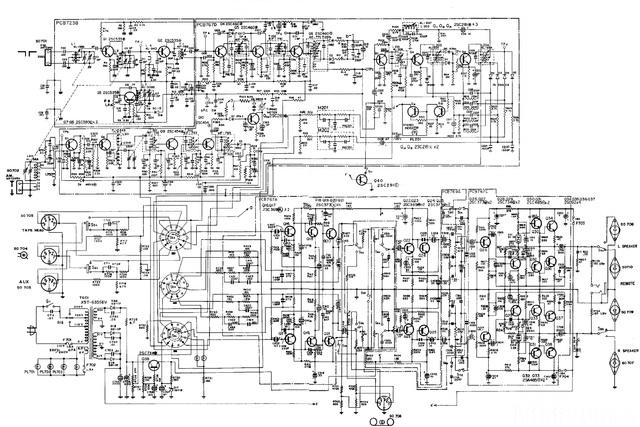
\includegraphics[width=0.80\textwidth]{pics/schaltplan_.jpg}
	\caption{Spannungsteiler basierte Ansteuerung einer LED}
	\label{fig:schaltplan}
\end{figure}
\\
\subsubsection{Verifikation}
Die Schaltung wird mit einer 0~V Quelle betrieben. .....\\
Messkurven, Foto,...
\\
\subsubsection{Auswertung}
Die LED leuchtet!!!!
\subsection{Zusammenfassung}


\section{Zusammenfassung}

\subsection{Erster interessanter Punkt}

\subsection{Und noch ein wichtiger Aspekt}

Hier werden die zuvor beschriebenen Ergebnisse diskutiert...
\section{Anhang}

Hier folgen plots, Simulationen etc welche nicht wesentlich sind.
\listoffigures
\listoftables
\bibliography{literatur}

\end{document}


